\documentclass[../main.tex]{subfiles} % ~1400 Worte

\begin{document}

\subsection{Benutzeranforderungen als Use Cases}

Bei der Entwicklung von Softwareprojekten, wie der Webanwendung `ShroomScout', ist die sorgfältige Definition von
Benutzeranforderungen ein entscheidender Schritt. Eine bewährte Strategie zur Strukturierung und Priorisierung dieser
Anforderungen ist die Erstellung von Use Cases. Use Cases beschreiben typische Interaktionen zwischen dem Nutzer und
dem System und dienen dazu, klare und nachvollziehbare Anforderungen zu formulieren. Im Folgenden werden die zentralen
Use Cases für `ShroomScout' detailliert beschrieben, um die grundlegenden Benutzeranforderungen zu veranschaulichen
(siehe Abbildung~\ref{fig:UseCase_Diagramm}).

\begin{figure}[ht]
	\centering
	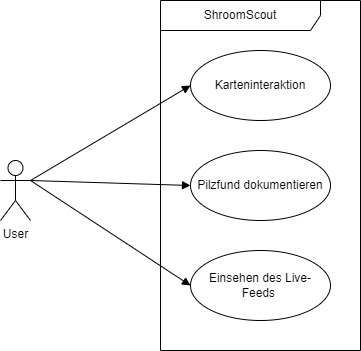
\includegraphics[width=0.5\textwidth]{abbildungen/UseCaseDiagrammDrawio.jpg}
	\caption{Use Cases von ShroomScout.}
	\label{fig:UseCase_Diagramm}
\end{figure}

\subsubsection{Karteninteraktion}

Die Karte ist das zentrale Element von `ShroomScout' und soll es den Nutzern ermöglichen, bereits eingetragene Pilzfundorte
visuell zu erfassen. Nutzer sollen auf der Karte navigieren können, indem sie hin- und herscrollen, sowie hinein- und herauszoomen,
um unterschiedliche Bereiche und Detailstufen zu erkunden. Diese Funktionen sind essenziell, um die Suche nach Pilzstandorten
intuitiv und effizient zu gestalten. Bereits eingetragene Pilzfundorte sollen mit einem Marker markiert sein und der Name des
dort gefundenen Pilzes soll durch anklicken oder hovern angezeigt werden können. Die Interaktion mit der Karte ist also in
Anlehnung an andere kartenbasierte Anwendungen konzipiert, sodass Nutzer leicht den gewünschten Kartenausschnitt oder
eingetragenen Pilz finden können, was eine hohe Benutzerfreundlichkeit der Anwendung ermöglichem soll.

\subsubsection{Pilzfund dokumentieren}

Ein weiterer zentraler Use Case ist das Eintragen eines Pilzfunds durch den Nutzer. Dieser Prozess beginnt mit dem Klick auf
die Schaltfläche `Pilz eintragen' und umfasst mehrere Schritte:

\begin{itemize}

	\item \textbf{Eingabe vom Pilznamen und dessen Umgebung:}
	      Der Nutzer gibt zunächst den Namen des Pilzes ein. Dies soll durch eine automatische Vervollständigung unterstützt werden,
	      um Tippfehler zu vermeiden und den Prozess zu beschleunigen. Zusätzlich wird die Umgebung des Pilzfunds (z.B. Wiese, Eiche)
	      erfasst, auswählbar aus einem Dropdown Menü.

	\item \textbf{Anzeigen eines Bildes des Pilzes:}
	      Nach der Eingabe des Pilznamens soll automatisch ein Bild des entsprechenden Pilzes angezeigt werden. Dies dient der visuellen
	      Bestätigung und hilft, Verwechslungen zu vermeiden.

	\item \textbf{Markieren des Fundorts auf der Karte:}
	      Der Nutzer platziert einen Marker auf der Karte, um den genauen Fundort des Pilzes zu dokumentieren. Diese Markierung soll
	      korrigierbar sein, falls Nutzer versehentlich den falschen Standort angeben.

	\item \textbf{Finale Dokumentation:}
	      Sind alle Informationen angegeben, soll der Pilzfundort mit einem Knopf eingetragen werden können. Um sicherzustellen, dass
	      alle notwendigen Eingaben getätigt worden sind, soll sich dieser erst aktivieren, wenn die drei oben stehenden Aktionen ausgeführt
	      worden sind. So kann es zu keinen fehlerhaften Einträgen kommen, was weiter zur Benutzerfreundlichkeit und Einfachheit beiträgt.

\end{itemize}

\subsubsection{Einsehen des Live-Feeds}

Der Live Feed stellt eine Auflistung der jüngsten Pilzfunde dar und soll kontinuierlich aktualisiert werden. Obwohl Nutzer mit dem
Live Feed nicht direkt interagieren können, dient er als wichtige Informations- und Inspirationsquelle für die Community. Die Anzeige
der neuesten Funde soll das Gemeinschaftsgefühl fördern und Nutzer motivieren, selbst an pilzreichen Orten Pilze suchen zu gehen. Obwohl
der Live Feed keine direkte Nutzerinteraktion beinhaltet, ist er ein wesentlicher Bestandteil des Nutzererlebnisses und trägt zur Dynamik
der Anwendung bei.

Zusammenfassend bilden diese Use Cases das Fundament für die Interaktion der Nutzer mit `ShroomScout' und definieren klare
Anforderungen an die Funktionalität und Benutzerfreundlichkeit der Anwendung. Durch die detaillierte Ausarbeitung dieser Use
Cases wird sichergestellt, dass die Entwicklung von `ShroomScout' den Bedürfnissen und Erwartungen der Zielgruppe entspricht
und eine intuitive, effiziente und ansprechende Benutzererfahrung bietet.

\subsection{Funktionale Anforderungen} % Tim

Funktionale Anforderungen definieren die spezifischen Verhaltensweisen und Funktionen, die ein Softwaresystem oder eine Anwendung ausführen muss, um die festgelegten Ziele und Bedürfnisse der Stakeholder zu erfüllen. 
Diese Anforderungen beschreiben detailliert, was das System tun soll, einschließlich der Prozesse, Datenmanipulationen, Benutzerinteraktionen und anderer erforderlicher Funktionen. 
Sie sind essentiell für die Entwicklung und Validierung eines Softwaresystems, da sie eine grundlegende Rolle in der Spezifikation der Softwarearchitektur und -design spielen und als Maßstab für die Überprüfung der Systemleistung und -funktionalität dienen. 
Funktionale Anforderungen müssen präzise, eindeutig, messbar, verifizierbar und realisierbar formuliert sein, um eine effektive Implementierung und Bewertung der Software zu gewährleisten. 
In der Literatur werden sie oft im Kontext von Anforderungsanalyse und Systemspezifikation diskutiert, um die Brücke zwischen den initialen Benutzerbedürfnissen und der technischen Umsetzung zu schlagen.
Einige Funktionale Anforderungen an Shroomscout sind im Folgenden aufgeführt:

\begin{itemize}

	\item \textbf{Registrieren eines Pilzfunds}
	      Der User muss die Möglichkeit haben einen neuen Pilzfund, über eine Eingabemaske im Frontend zu registrieren.
		  Diese Eingabemaske soll eine automatische Vervollständigung der Eingabe anbieten und soll bereits validieren ob die Eingabe einem gültigen
		  Wert entspricht. Die in die Eingabemaske einzugebenden Daten sind die Art des Pilzes sowie die Umgebung in der er gefunden wurde.
		  Erst wenn ein Marker für den Standort auf der Karte gesetzt und sowohl für Art und Umgebung des Pilzes valide Werte eingetragen wurden, soll es 
		  möglich sein den Eintrag zu speichern, davor soll der Button zum registrieren ausgegraut sein.

	\item \textbf{Anzeigen eines Live Feeds}
	      Es soll auf der Startseite einen Livefeed geben in dem die letzten Pilzfunde geben. 
		  Aus dem Livefeed sollen Art und Umgebung der zuletzt registrierten Pilze hervorgehen

	\item \textbf{Anzeige der registrierten Pilze}
		  Die registrierten Pilze sollen auf einer Openstreetmap Karte als Marker angezeigt werden.
		  Wenn die Marker angeklickt werden sollen zusätzliche Informationen wie die Art des Pilzes angezeigt werden.
	      

	\item \textbf{Navbar}
	      Die Navbar soll die Navigation der Seite ermöglichen und die Möglichkeit bieten, die Eingabemaske zum Registrieren eines Pilzes zu öffnen, sowie zur Startseite zurückzukehren.
		  Die Navbar soll blau sein und am linken Bildschirmrand das Shroomscout Logo beinhalten

	\item \textbf{Design}
	      Um eine einheitliche Erfahrung zu schaffen und die Wartung zu erleichtern, sollen primär Komponenten der von Google verwalteten Angular Materials Library verwendet werden.

\end{itemize}


\subsection{Nicht-funktionale Anforderungen}

Neben den funktionalen Anforderungen, die spezifische Aktionen und Verhaltensweisen des Systems beschreiben, spielen
nicht-funktionale Anforderungen eine entscheidende Rolle für den Erfolg eines Softwareprojekts. Sie definieren die
Qualitätsattribute der Anwendung und beeinflussen maßgeblich die Nutzerzufriedenheit. Für die Webanwendung `ShroomScout'
sind die folgenden nicht-funktionale Anforderungen eingeplant:

\begin{itemize}

	\item \textbf{Einfachheit und Benutzerfreundlichkeit}
	      `ShroomScout' soll durch eine intuitive Bedienbarkeit bestechen. Die Anwendung muss so gestaltet sein, dass Nutzer mit
	      minimalen Aufwand und ohne Vorkenntnisse die Kernfunktionalitäten nutzen können. Dazu gehört eine klare und verständliche
	      Nutzeroberfläche, die es dem Anwender ermöglicht, ohne umständliche Navigation oder komplizierte Prozesse Pilze zu finden
	      und einzutragen.

	\item \textbf{Responsive Design}
	      Angesichts der Tatsache, dass Nutzer `ShroomScout' häufig im Freien und damit auf mobilen Geräten nutzen werden, ist ein
	      responsive Design unerlässlich. Das heißt, dass sich die Anwendung automatisch an verschiedene Bildschirmgrößen und -auflösungen
	      anpassen muss, um auf Smartphones, Tablets und Desktop-Computern gleichermaßen gut bedienbar zu sein. Dies gewährleistet eine
	      optimale Benutzererfahrung unabhängig vom Endgerät.

	\item \textbf{Schnelle Ladezeiten}
	      Für eine positive Nutzererfahrung sind kurze Ladezeiten von großer Bedeutung. `ShroomScout' sollte so optimiert sein, dass die
	      Anwendung auch bei langsamer Internetverbindung schnell lädt, bzw. aktualisiert. Dies ist besonders wichtig, da Nutzer die Anwendung
	      möglicherweise in Gebieten mit schlechter Netzabdeckung verwenden.

	\item \textbf{Sicherheit und Datenschutz}
	      Die Sicherheit persönlicher Daten und die Wahrung der Privatsphäre der Nutzer sind essenzielle Anforderungen. `ShroomScout'
	      muss sicherstellen, dass alle Nutzerdaten, insbesondere Standortinformationen und persönliche Informationen, gemäß den
	      geltenden Datenschutzrichtlinien behandelt und geschützt werden.

	\item \textbf{Skalierbarkeit}
	      Die Anwendung muss in der Lage sein, mit einer zunehmenden Anzahl von Nutzern und Datenmengen zu skalieren. Dies stellt
	      sicher, dass `ShroomScout' auch bei wachsender Beliebtheit und steigenden Anforderungen stabil und performant bleibt.

\end{itemize}

Durch die Berücksichtigung dieser nicht-funktionalen Anforderungen in der Entwicklungsphase wird sichergestellt, dass `ShroomScout'
nicht nur funktionell den Bedürfnissen der Nutzer entspricht, sondern auch in Bezug auf Qualität und Benutzerfreundlichkeit überzeugt.

\end{document}
